%----------------------------------------------------------------------------------------
\chapter{Platforms}
\label{chap:platforms}
%----------------------------------------------------------------------------------------
In this chapter, all the physical and digital platforms utilized will be explained to give a proper understanding of the initial architecture and a more comprehensive idea of the environment of the experiments. The first part will state the devices and their setup, capabilities, and configuration used. Subsequently, the frameworks and libraries employed will be listed and described. 

\section{Baxter Robot}
The Baxter robot is an industrial robot built by Rethink Robotics in 2011 \cite{wiki:baxter}. The platform [Fig. \ref{fig:baxter}] has two robotic arms with interchangeable grippers at the wrist (End Effectors). The robot is 180cm tall and, with its pedestal, weighs 140 kg. The arms have 7 degrees of freedom (DOF), which implies they have seven joints each. This makes it kinematic redundant, meaning that for some points reached in space, multiple pose configurations of the arms are possible. These two factors combined allow the robot to have an impressive capability in manipulation. The robot can be equipped with suction caps or two-jaw parallel grippers; we chose the last ones in our configuration. The gripper, in addition to its position, also offers information regarding the force applied while grasping an object.

The robot was designed with attention to collaborative tasks with humans. For this reason, it eases teaching by demonstration by having integrated two touch sensors in the wrists that unlock the motors of the arms, allowing the user to move them easily and record the trajectories executed. The robot helps the movement with a feature called "Zero-g mode", in which the weight of the joints is neutralized actively by the motors. This enables the teaching expert to demonstrate movements in a similar environment without gravity, without having to carry the instrumentation load in time constantly. Furthermore, the robot has many input buttons and LEDs, they are present on the hands, arms, and chest, and they allow the programming of custom behaviors. They are especially useful in retrieving and giving instructions to the robot without reaching a computer, like closing the gripper at the desired moment, getting feedback, or starting the trajectory recordings. 

Another feature worth mentioning is the increased safety of operating around humans. Thanks to active and passive safety systems equipped in the platform, it doesn't require a cage for protection. On the other hand, making the robot less hazardous comes with the cost of precision. A motor driving a spring that drives Baxter's arm instead of just a direct motor impacts the precision of movements, sometimes in terms of centimeters. This doesn't make the robot perfectly suitable for industrial applications, but especially appropriate for research and for the adaptability in our project.

The head of the robot includes a ring of sonar sensors for people detection, a wide-angle camera, and a movable display that acts like a face. 
Another benefit of the robot lies at the end of both hands. Immediately next to the attachment for the tools, an infrared (IR) sensor provides data on the distance from a solid object (i.e., a table) and an inertial measurement unit (IMU). Moreover, an embedded RGB camera is also present, allowing to see closely the object approached or to change the point of view on it without additional external cameras.

\begin{figure}
	\centering
	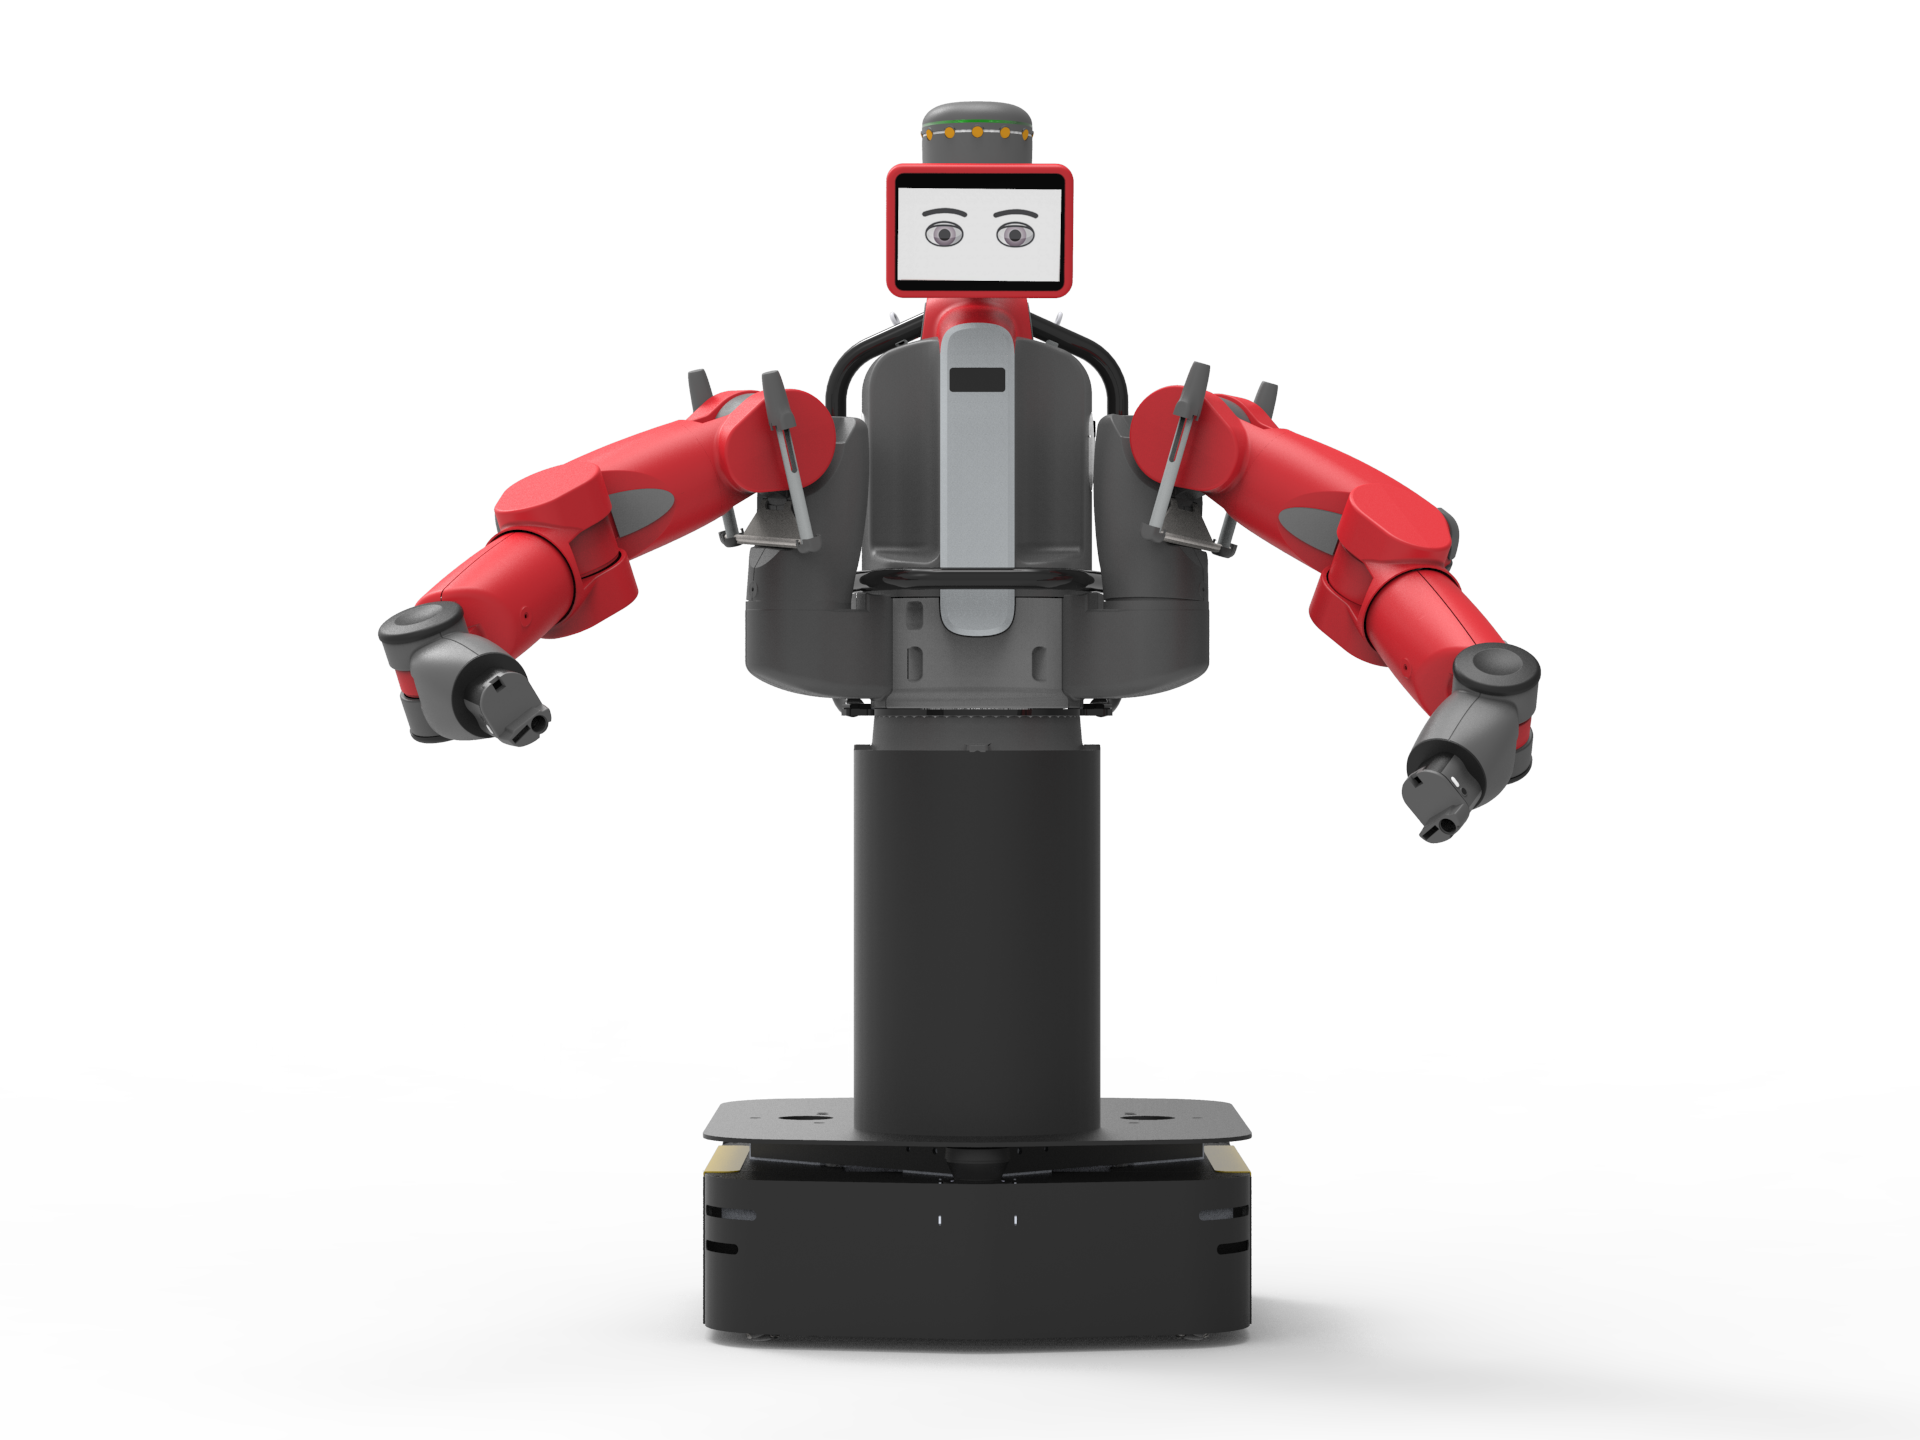
\includegraphics[width=0.5\linewidth]{Images/baxter.png}
	\caption{Baxter Robot platform}
	\label{fig:baxter}
\end{figure}

\section{UR10 Robot}
UR10 is a single industrial robot arm that shines in reliability and precision [Fig. \ref{fig:ur10}]. It has been manufactured by Universal Robots and combines long reach with a high payload \cite{url:ur10}. It is intended for medium-duty tasks, so it's compact in its overall dimensions compared to a fully intended industrial robot. It can reach an impressive height of 2.3m on its pedestal. In our experiments, it was mounted on a pedestal 0.85m tall to increase the reachability at table level. 

The arm has a reaching radius of 1,3m from the mounting point, which implies a workspace of approximately 5,3 square meters at the base level. The robot has 6 Degrees of Freedom, with six rotating joints. It is able to reach any point in its reaching radius but has no kinematics redundancy, meaning only one position is possible for any given point. The total payload that can be carried is 10 kg. 

\begin{figure}
	\centering
	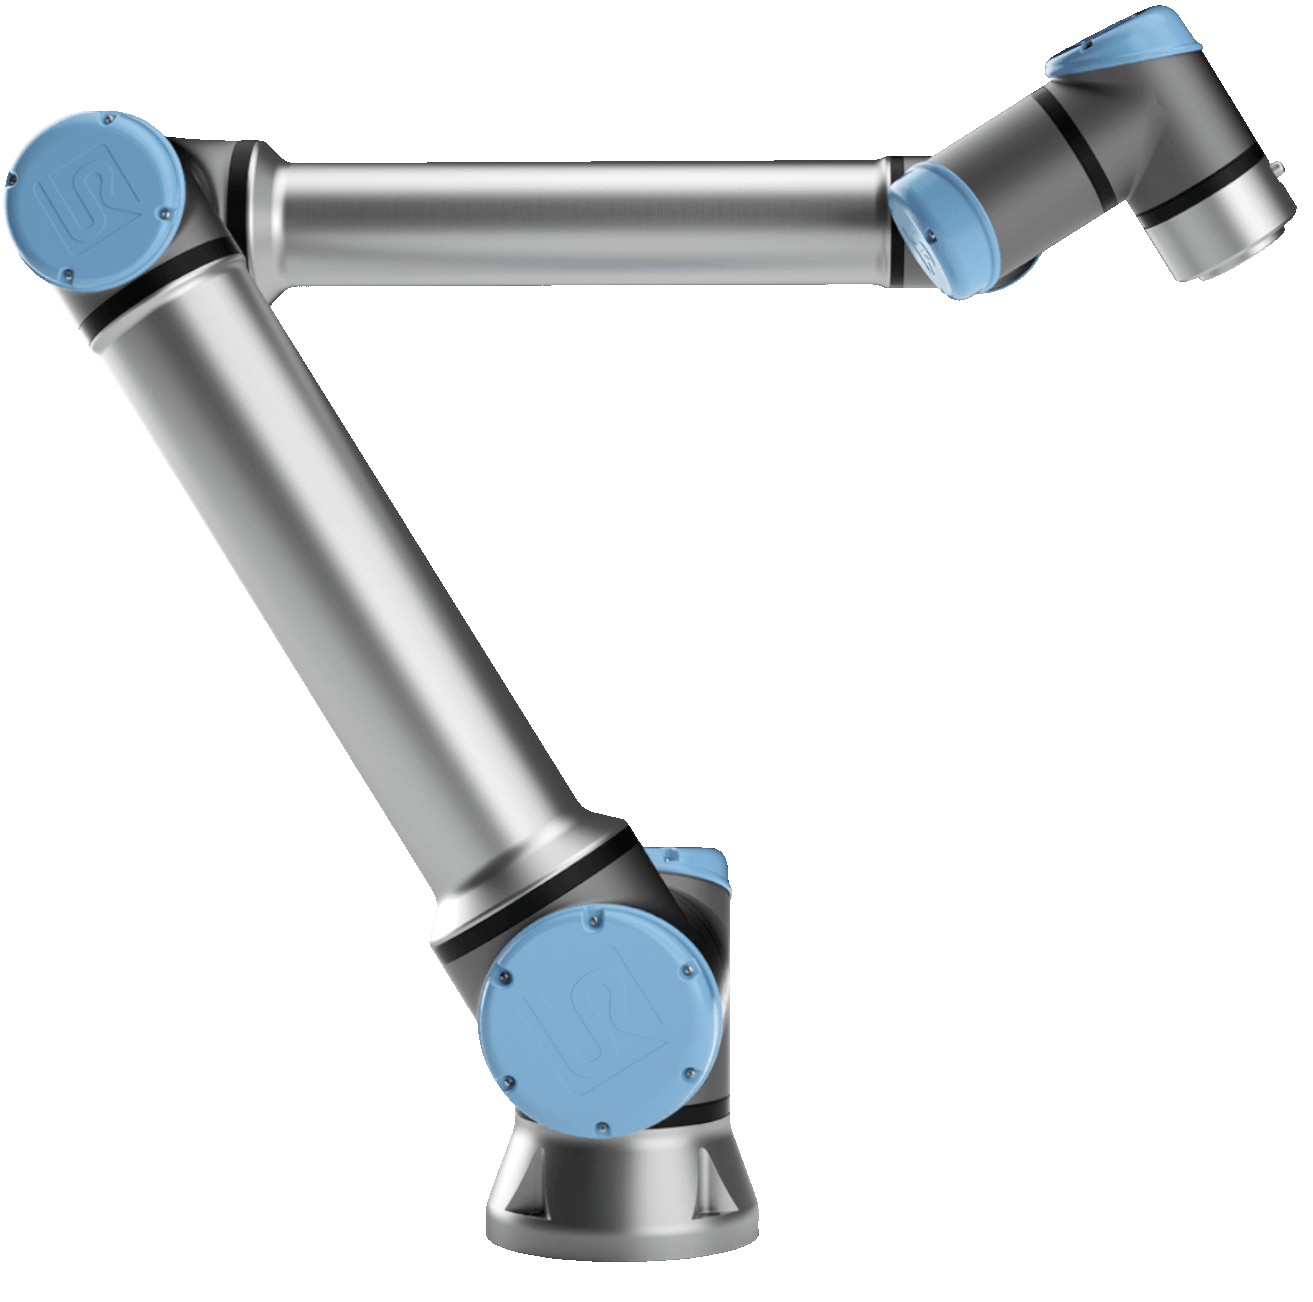
\includegraphics[width=0.5\linewidth]{Images/ur10.png}
	\caption{UR10 Robot platform}
	\label{fig:ur10}
\end{figure}

Like the previous robot, this one is designed to work collaboratively with humans. It features built-in safety features, such as force/torque sensors, to detect and respond to external forces or unexpected events. A button to release the motor breaks is present on the floating touch screen and allows the robot's motion by hand. This robot also doesn't require a safety cage around for protection, but the emergency stop button always has to be within easy reach. 

The robot design emphasizes modularity, making it easier for users to customize and adapt it for different tasks or use various end effectors. We coupled it with a three-finger gripper described in the next paragraph.


\section{3F Robotiq Gripper}
At the end of the UR10 Robotic Arm, a Robotiq 3-Finger Adaptive Robot Gripper was mounted [Fig. \ref{fig:gripper3f}]. The gripper has a human-inspired design and has three fingers with three joints each \cite{url:3fgripper}. The physical platform was chosen for its precision and safety, and it pairs well with the UR10 capabilities. The gripper offers different grip modes; the ones available are: "basic", "wide", "scissor" and "pinch". Each is appropriate for distinctive objects to grip; the basic one is the most versatile, but the wide one has more stability for big or long objects, and the pinch one is the best for small objects. The "scissor mode" closes together the two fingers on the same side, for high-precision manipulation. We mainly used the "pinch" setting. 

\begin{figure}
	\centering
	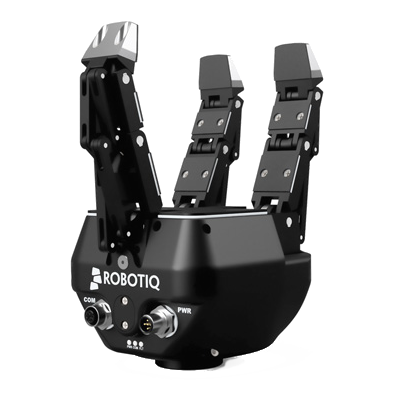
\includegraphics[width=0.5\linewidth]{Images/gripper3f.png}
	\caption{3F Robotiq Gripper platform}
	\label{fig:gripper3f}
\end{figure}

The gripper has a mass of 2.3 kg in contrast with a grip payload of 10 kg. The grip force applied can range from 30 to 70 N, depending on the grip mode selected. The precision declared is up to 0.05 mm.

This platform was designed as well for collaborative robotic applications, allowing it to work safely alongside human operators. It incorporates safety features to detect and respond to external forces, stopping in case of high forces applied. The torque and speed of gripping data are available and exposed through a dedicated ROS topic. Speed and torque are also adjustable for the intended use. It is possible to control and retrieve data for each finger individually. 



\section{FT 300-S Force Torque Sensor}
Between the UR10 robot and the 3F Finger Gripper, an FT 300-S Force Torque Sensor [Fig. \ref{fig:ft-sensor}] was mounted to increase precision and repeatability. 

The sensor offers high-resolution real-time measurements regarding the force and torque applied to the three space dimensions and improves the capabilities of the robot. This device makes the UR10 able to detect the payload carried or the amount of pressure between the object or gripper and the static environment (i.e., the table). 

The device was built for compatibility with the Universal Robot series and has an IP65 rating. It also enables precise object placement such as alignment, indexing, and insertion \cite{url:ftsensor}. 

It exposes the six readings of the forces and torques in the three axes through a port opened in the computer connected to it. In out setup it has been connected straight to the UR10 computer, allowing any user to retrieve the necessary data.  

The FT 300-S is commonly used in tasks where force and torque sensing are critical, but we used it to increase the reliability of the payload measurements and the safety of the operations. 

\begin{figure}
	\centering
	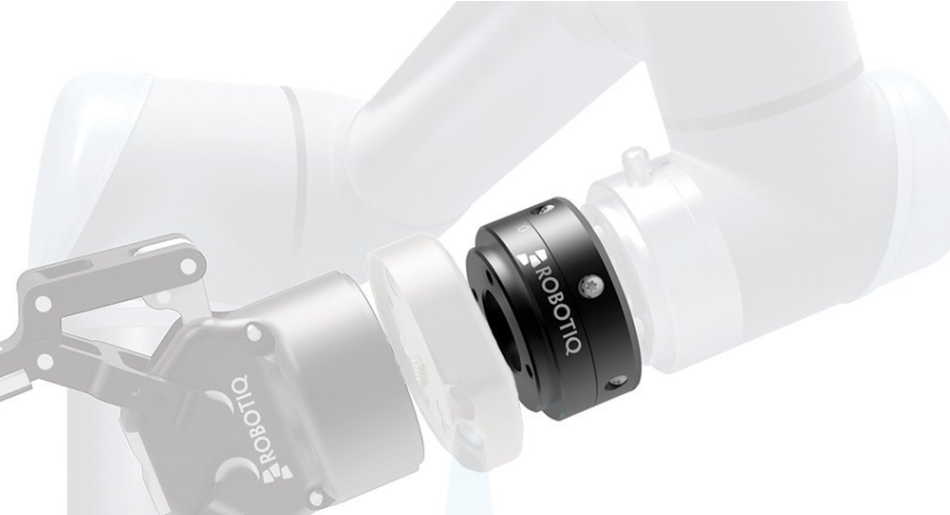
\includegraphics[width=0.9\linewidth]{Images/ft_sensor.png}
	\caption{FT 300-S Force Torque Sensor}
	\label{fig:ft-sensor}
\end{figure}

\newpage
\section{Frameworks}
\paragraph{ROS}
The Robot Operating System (ROS) \cite{url:ros} is a framework to standardize the deployment of robot applications. The system is a set of software libraries and tools that combine the state-of-the-art drivers for the most common robot interfaces and contain the most used algorithms for robotics. 

Since robotics programming is a complex challenge, the idea behind ROS is to use the "divide et impera" approach and split it into multiple sub-problems. This division requires a distributed strategy, and distribution implies communication among parts. One of ROS's main objectives is to standardize communication. For this reason, ROS acts like a middleware framework, allowing the ease of the dialog between software and the robotic hardware. It is widely used in research and industry, from mobile robots to manipulators. In our research, we used ROS version 1. 

It's platform-independent and open source, so it is possible to create a custom robotics device compatible with it, and it's possible to develop personalized libraries. Its modular architecture allows the creation or use of a series of executable pieces of code called nodes, which run on a single or even on many computers. The nodes communicate among themselves with messages in the form of data structures previously defined. The distributed system allows to decuple the computation of heavy tasks, like vision, 3D reconstruction, and navigation, from the robot's hardware. 

Communication occurs through "topics" and "services". Nodes running on any computer ping the "master node" designated to retrieve all the possible topics and services exposed from other nodes in the network. A node can be a "publisher" or "subscriber" to a topic, sending messages to it or receiving messages from it. Communication with topics is not blocking and it is many-to-many: multiple nodes can publish, and simultaneously, multiple nodes can subscribe to a topic. Services work in a similar way, but the communication blocks the computation till the data requested is retrieved. Their mechanism is analogous to Remote Procedure Calls (RPCs). 

ROS is available with two commonly used programming languages: Python and C++. We used the Python version with the "rospy" package in the experiments with both robots.

\paragraph{Pytorch}
Pytorch is a Deep Learning framework \cite{paszke2019pytorch} that focuses on speed and usability with an imperative and Pythonic programming style.  The Python library \cite{url:pytorch} offers a wide variety of models and building blocks for constructing neural networks. By design, it eases the debugging for the user with a rich ecosystem of dedicated tools. It works on the CPU and on hardware accelerators like GPUs. For this reason, PyTorch provides a multi-dimensional array called a tensor, which is similar to NumPy arrays. Conversions among both of them will be present in the code implementation. 

\paragraph{Jupyter Notebook}
Jupyter Notebook is an open-source interactive web application \cite{url:jupyter}. It supports multiple programming languages and offers a cell-based environment where code and description/graphical results can be blended. Jupyter Notebook integrates seamlessly with popular Python libraries, such as NumPy, Pandas, Matplotlib, and scikit-learn; some of them will be described later. It was used occasionally in our experiments to provide a fast and interactive coding experience with Python. The notebooks can be easily shared, and the process is clearly visualized. It was specifically useful in plotting multiple graphs during the training stages of neural networks or debugging operations on multi-dimensional arrays. 

\paragraph{Anaconda and Python Libraries}
Anaconda is an open-source software that contains open-source tools and packages for data science, machine learning, and scientific computing \cite{url:anaconda}. It has been used to track the packages utilized in the robotic platforms and in the models' development and training. The Conda package manager was the most used tool to easily install, update, and manage various software packages and dependencies. Some of the most important libraries are listed below.
\subparagraph{MatplotLib} Matplotlib is a comprehensive 2D plotting library for Python that generates high-quality charts, plots, and visualizations. It has been widely used to double-check the quality of the training or plot the trajectories recorded with the robots. 
\subparagraph{Numpy} NumPy is a package for numerical computing in Python. It supports large, multi-dimensional arrays and matrices and a collection of mathematical functions to operate on these arrays. It has been used for array slicing, normalization, and smoothing data. 